\chapter{Unit Benchmarks}
\epigraphhead[120]{\epigraph{Any intelligent fool can make things bigger, more complex, and more violent. It takes a touch of genius -- and a lot of courage -- to move in the opposite direction.}{\textit{Albert Einstein}}}




\section{Examples}
\begin{myDefinition}{Stability and Condition}{stabAndCondi}
	Let $F : \mathbb{R}^n \to \mathbb{R}^m$ be the problem which depends on $x$ and $\widetilde F$ should be the numerical algorithm which approximates the problem. $\widetilde x$ is the disturbed input data.
	
	In order to estimate the error we can use the triangle inequality:
	\begin{align}
	\left\| F\left(x\right) - \widetilde F\left(\widetilde x\right) \right\| \leq \underbrace{\left\| \vphantom{\widetilde F} F\left(x\right) - F\left(\widetilde x\right) \right\|}_\mathrm{condition}  + \underbrace{\left\| F\left(\widetilde x\right) - \widetilde F\left(\widetilde x\right) \right\|}_\mathrm{stability} \text{.}
	\end{align}
	Note that condition is a property of the problem itself and stability is a property of the algorithm.
\end{myDefinition}


\begin{algorithm}[!htb]
	\DontPrintSemicolon
	\LinesNumbered
	\tcp*[l]{Initialize}
	
	${^{0}}\vectorsym{x} = {^{\mathrm{init} }}\vectorsym{x}$
	
	\tcp*[l]{Iteration loop}\For{$m=0$ to $m=m_{\mathrm{end}}$}{ 
		
		\tcp*[l]{Evaluate and check residual}
		
		$\leftidx{^{m}}{\vectorsym{r}} = F\left( {^{m}} \vectorsym{x} \right)$
		
		\If{$\left\| \leftidx{^{m}}{\vectorsym{r}} \right\|_{\mathrm{\epsilon}}<\epsilon$}{
			break\;
		}
		
		\tcp*[l]{Evaluate Jacobian}
		
		${}^{m}\matrixsym{J}_{}^{}= \mathcal J\left(F\left({^{m}}\vectorsym{x} \right) \right) $
		
		\tcp*[l]{Solve for corrector}
		
		${}^{m}\matrixsym{J}_{\mathrm{}}^{} \cdot {}^{m} \Delta \vectorsym{x} = -{}^{m}\vectorsym{r}^{}$
		
		
		\tcp*[l]{Apply update}		
		${^{m+1}}\vectorsym{x} = {^{m}}\vectorsym{x} + {^{m}} \Delta \vectorsym{x}$
		
		
	}
	
	\caption{Ordinary Newton method for vector case}
	\label{alg:ordNewton}
\end{algorithm}

\begin{table}[!htb]
	\caption{Test table}
	\begin{center}
		\begin{tabular}{@{}n{1}{0} n{1}{16} n{1}{16} n{1}{16}@{}}\toprule
			\multicolumn{1}{@{}H}{iteration}& \multicolumn{1}{H}{$\left\| F\left(\leftidx{^{m}}x \right) \right\|$}& \multicolumn{1}{H}{$\left\|  \leftidx{^{m}} \Delta x \right\|$} & \multicolumn{1}{H@{}}{$\leftidx{^{m}}e_{\mathrm{fixP}}$} \tabularnewline\midrule\addlinespace
			%  &                     &                    &                    \tabularnewline\midrule\addlinespace
			0 & 1.4142135623730951  & 1.4142135567740073 & 0.3034928222344159 \tabularnewline
			1 & 0.4259168225819227  & 0.3082392919753713 & 0.0047464697409562 \tabularnewline
			2 & 0.0067125092788733  & 0.0047464875528316 & 0.0000000178118777 \tabularnewline
			3 & 0.0000000251897958  & 0.0000000180575680 & 0.0000000029776933 \tabularnewline\addlinespace\bottomrule
		\end{tabular}
	\end{center}
	\label{tab:JFNK}
\end{table}


\begin{figure}[H]
	\centering
	% GNUPLOT: LaTeX picture with Postscript
\begingroup
  % Encoding inside the plot.  In the header of your document, this encoding
  % should to defined, e.g., by using
  % \usepackage[cp1252,<other encodings>]{inputenc}
  \inputencoding{cp1252}%
  \makeatletter
  \providecommand\color[2][]{%
    \GenericError{(gnuplot) \space\space\space\@spaces}{%
      Package color not loaded in conjunction with
      terminal option `colourtext'%
    }{See the gnuplot documentation for explanation.%
    }{Either use 'blacktext' in gnuplot or load the package
      color.sty in LaTeX.}%
    \renewcommand\color[2][]{}%
  }%
  \providecommand\includegraphics[2][]{%
    \GenericError{(gnuplot) \space\space\space\@spaces}{%
      Package graphicx or graphics not loaded%
    }{See the gnuplot documentation for explanation.%
    }{The gnuplot epslatex terminal needs graphicx.sty or graphics.sty.}%
    \renewcommand\includegraphics[2][]{}%
  }%
  \providecommand\rotatebox[2]{#2}%
  \@ifundefined{ifGPcolor}{%
    \newif\ifGPcolor
    \GPcolortrue
  }{}%
  \@ifundefined{ifGPblacktext}{%
    \newif\ifGPblacktext
    \GPblacktextfalse
  }{}%
  % define a \g@addto@macro without @ in the name:
  \let\gplgaddtomacro\g@addto@macro
  % define empty templates for all commands taking text:
  \gdef\gplbacktext{}%
  \gdef\gplfronttext{}%
  \makeatother
  \ifGPblacktext
    % no textcolor at all
    \def\colorrgb#1{}%
    \def\colorgray#1{}%
  \else
    % gray or color?
    \ifGPcolor
      \def\colorrgb#1{\color[rgb]{#1}}%
      \def\colorgray#1{\color[gray]{#1}}%
      \expandafter\def\csname LTw\endcsname{\color{white}}%
      \expandafter\def\csname LTb\endcsname{\color{black}}%
      \expandafter\def\csname LTa\endcsname{\color{black}}%
      \expandafter\def\csname LT0\endcsname{\color[rgb]{1,0,0}}%
      \expandafter\def\csname LT1\endcsname{\color[rgb]{0,1,0}}%
      \expandafter\def\csname LT2\endcsname{\color[rgb]{0,0,1}}%
      \expandafter\def\csname LT3\endcsname{\color[rgb]{1,0,1}}%
      \expandafter\def\csname LT4\endcsname{\color[rgb]{0,1,1}}%
      \expandafter\def\csname LT5\endcsname{\color[rgb]{1,1,0}}%
      \expandafter\def\csname LT6\endcsname{\color[rgb]{0,0,0}}%
      \expandafter\def\csname LT7\endcsname{\color[rgb]{1,0.3,0}}%
      \expandafter\def\csname LT8\endcsname{\color[rgb]{0.5,0.5,0.5}}%
    \else
      % gray
      \def\colorrgb#1{\color{black}}%
      \def\colorgray#1{\color[gray]{#1}}%
      \expandafter\def\csname LTw\endcsname{\color{white}}%
      \expandafter\def\csname LTb\endcsname{\color{black}}%
      \expandafter\def\csname LTa\endcsname{\color{black}}%
      \expandafter\def\csname LT0\endcsname{\color{black}}%
      \expandafter\def\csname LT1\endcsname{\color{black}}%
      \expandafter\def\csname LT2\endcsname{\color{black}}%
      \expandafter\def\csname LT3\endcsname{\color{black}}%
      \expandafter\def\csname LT4\endcsname{\color{black}}%
      \expandafter\def\csname LT5\endcsname{\color{black}}%
      \expandafter\def\csname LT6\endcsname{\color{black}}%
      \expandafter\def\csname LT7\endcsname{\color{black}}%
      \expandafter\def\csname LT8\endcsname{\color{black}}%
    \fi
  \fi
    \setlength{\unitlength}{0.0500bp}%
    \ifx\gptboxheight\undefined%
      \newlength{\gptboxheight}%
      \newlength{\gptboxwidth}%
      \newsavebox{\gptboxtext}%
    \fi%
    \setlength{\fboxrule}{0.5pt}%
    \setlength{\fboxsep}{1pt}%
\begin{picture}(7200.00,5040.00)%
    \gplgaddtomacro\gplbacktext{%
      \colorrgb{0.00,0.00,0.00}%%
      \put(948,756){\makebox(0,0)[r]{\strut{}$0$}}%
      \colorrgb{0.00,0.00,0.00}%%
      \put(948,1428){\makebox(0,0)[r]{\strut{}$5$}}%
      \colorrgb{0.00,0.00,0.00}%%
      \put(948,2100){\makebox(0,0)[r]{\strut{}$10$}}%
      \colorrgb{0.00,0.00,0.00}%%
      \put(948,2772){\makebox(0,0)[r]{\strut{}$15$}}%
      \colorrgb{0.00,0.00,0.00}%%
      \put(948,3443){\makebox(0,0)[r]{\strut{}$20$}}%
      \colorrgb{0.00,0.00,0.00}%%
      \put(948,4115){\makebox(0,0)[r]{\strut{}$25$}}%
      \colorrgb{0.00,0.00,0.00}%%
      \put(948,4787){\makebox(0,0)[r]{\strut{}$30$}}%
      \colorrgb{0.00,0.00,0.00}%%
      \put(1080,536){\makebox(0,0){\strut{}$0$}}%
      \colorrgb{0.00,0.00,0.00}%%
      \put(1920,536){\makebox(0,0){\strut{}$5$}}%
      \colorrgb{0.00,0.00,0.00}%%
      \put(2760,536){\makebox(0,0){\strut{}$10$}}%
      \colorrgb{0.00,0.00,0.00}%%
      \put(3600,536){\makebox(0,0){\strut{}$15$}}%
      \colorrgb{0.00,0.00,0.00}%%
      \put(4439,536){\makebox(0,0){\strut{}$20$}}%
      \colorrgb{0.00,0.00,0.00}%%
      \put(5279,536){\makebox(0,0){\strut{}$25$}}%
      \colorrgb{0.00,0.00,0.00}%%
      \put(6119,536){\makebox(0,0){\strut{}$30$}}%
    }%
    \gplgaddtomacro\gplfronttext{%
      \csname LTb\endcsname%%
      \put(464,2771){\rotatebox{-270}{\makebox(0,0){\strut{}Difference level D [dB]}}}%
      \put(3599,206){\makebox(0,0){\strut{}Stiffness Ratio}}%
      \csname LTb\endcsname%%
      \put(5132,4614){\makebox(0,0)[r]{\strut{}$ 20 \cdot \log \left| \nicefrac{v_o}{v_u} \right| $}}%
      \csname LTb\endcsname%%
      \put(5132,4394){\makebox(0,0)[r]{\strut{}$ 20 \cdot \log \left| \nicefrac{\left(k_1 + k_2\right)}{k_1}\right| $}}%
    }%
    \gplbacktext
    \put(0,0){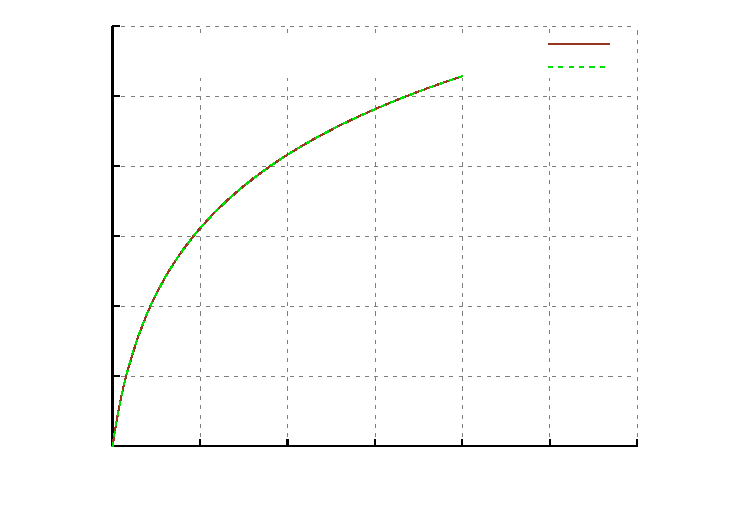
\includegraphics{insulationZeller2Dof}}%
    \gplfronttext
  \end{picture}%
\endgroup

	\caption{Difference level over stiffness ratio for 2DOF Mass oscillator}
	\label{fig:DoverRatio}
\end{figure}

\begin{figure}[!htb]
	\centering
	\def\svgwidth{0.6\textwidth}
	\input{unittests/fig/template.pdf_tex}
	\caption{template}
	\label{fig:template}
\end{figure}

\begin{landscape}
\section{Tabular Overview}
\def\arraystretch{1}
\begin{center}
	\begin{longtable}{p{1cm} p{2cm}  p{21cm} p{1cm}}\toprule
           \#  & Catagory            & Description        & Page\tabularnewline\midrule\addlinespace		
			\rowcolor{TUMhellblau}
			\multicolumn{4}{l}{Sensor \& Environment Modelling} \tabularnewline
			\rowcolor{TUMhellhellhellblau}
			\multicolumn{4}{l}{Radar} \tabularnewline
			\rowcolor[gray]{.9}
			3 & 0.00  & 0.0047464875528316 & 45 \tabularnewline
			3 & 0.00  & 0.0047464875528316 & 45 \tabularnewline
			\rowcolor{TUMhellhellhellblau}
			\multicolumn{4}{l}{Camera} \tabularnewline
			\rowcolor[gray]{.9}
			3 & 0.00  & 0.0047464875528316 & 45 \tabularnewline
			3 & 0.00  & 0.0047464875528316 & 45 \tabularnewline
			\rowcolor{TUMhellhellhellblau}
			\multicolumn{4}{l}{Lidar} \tabularnewline
			\rowcolor[gray]{.9}
			3 & 0.00  & 0.0047464875528316 & 45 \tabularnewline
			3 & 0.00  & 0.0047464875528316 & 45 \tabularnewline
			\rowcolor{TUMhellhellhellblau}
			\multicolumn{4}{l}{Ultrasonic} \tabularnewline
			\rowcolor[gray]{.9}
			3 & 0.00  & 0.0047464875528316 & 45 \tabularnewline
			4 & 0.00  & 0.0000000180575689 & 12 \tabularnewline
			\rowcolor{TUMhellblau}
			\multicolumn{4}{l}{Vehicle Dynamics} \tabularnewline
			\rowcolor{TUMhellhellhellblau}
			\multicolumn{4}{l}{Tire model} \tabularnewline
			\rowcolor[gray]{.9}
			3 & 0.00  & 0.0047464875528316 & 45 \tabularnewline
			4 & 0.00  & 0.0000000180575689 & 12 \tabularnewline
			\rowcolor{TUMhellhellhellblau}
			\multicolumn{4}{l}{Vehicle Model} \tabularnewline
			\rowcolor[gray]{.9}
			3 & 0.00  & 0.0047464875528316 & 45 \tabularnewline
			4 & 0.00  & 0.0000000180575689 & 12 \tabularnewline
			\rowcolor{TUMhellhellhellblau}
			\multicolumn{4}{l}{Drivetrain Model} \tabularnewline
			\rowcolor[gray]{.9}
			3 & 0.00  & 0.0047464875528316 & 45 \tabularnewline
			4 & 0.00  & 0.0000000180575689 & 12 \tabularnewline
			\rowcolor{TUMhellblau}
			\multicolumn{4}{l}{Electronic Control Unit Modelling} \tabularnewline
			\rowcolor{TUMhellhellhellblau}
			\multicolumn{4}{l}{FMU} \tabularnewline
			\rowcolor[gray]{.9}
			3 & 0.00  & 0.0047464875528316 & 45 \tabularnewline
			4 & 0.00  & 0.0000000180575689 & 12 \tabularnewline
			\rowcolor{TUMhellblau}
			\multicolumn{4}{l}{Scenario Modelling} \tabularnewline
			\rowcolor{TUMhellhellhellblau}
			\multicolumn{4}{l}{File-Based (OpenSCENARIO)} \tabularnewline
			\rowcolor[gray]{.9}
			3 & 0.00  & 0.0047464875528316 & 45 \tabularnewline
			4 & 0.00  & 0.0000000180575689 & 12 \tabularnewline
			\rowcolor{TUMhellhellhellblau}
			\multicolumn{4}{l}{Data-Based (Data->Scenario)} \tabularnewline
			\rowcolor[gray]{.9}
			3 & 0.00  & 0.0047464875528316 & 45 \tabularnewline
			4 & 0.00  & 0.0000000180575689 & 12 \tabularnewline
			\rowcolor{TUMhellhellhellblau}
			\multicolumn{4}{l}{Key Performance Indicators} \tabularnewline
			\rowcolor[gray]{.9}
			3 & 0.00  & 0.0047464875528316 & 45 \tabularnewline
			4 & 0.00  & 0.0000000180575689 & 12 \tabularnewline
			\rowcolor{TUMhellblau}
			\multicolumn{4}{l}{Electronic Control Unit Modelling} \tabularnewline
			\rowcolor{TUMhellhellhellblau}
			\multicolumn{4}{l}{FMU} \tabularnewline
			\rowcolor[gray]{.9}
			3 & 0.00  & 0.0047464875528316 & 45 \tabularnewline
			4 & 0.00  & 0.0000000180575689 & 12 \tabularnewline\addlinespace\bottomrule
			\caption{Benchmark Table}
	\end{longtable}
\end{center}
\end{landscape}

